%% entwurf.tex
%% $Id: entwurf.tex 28 2007-01-18 16:31:32Z bless $
%%
%% ==============================
\chapter{Konzeption}
\label{ch:Design}
In diesem Kapitel werden die Anforderungen an die Forscherplattform und den hierfür benötigten Therapiemodellierungsansatz beleuchtet. Für diese werden zunächst die Persona dargestellt. Diese beschreiben verschiedene Eigenschaften der Personengruppen, die später den \emph{TherapyBuilder} bedienen, der in Kapitel \ref{ch:Background}  beschriebenen wird. Anschließend werden verschiedene Studien betrachtet, die von Psychologen entwickelt wurden. Die Studien bestehen aus Therapien, die beispielsweise auf ihre Wirksamkeit geprüft werden. Aus den Defiziten der Technologien, die im Stand der Technik diskutiert werden, den dargestellten Persona und den Studieneingenschaften, werden die Anforderungen an den Therapiemodellierungsansatz entwickelt. Auf Basis der Anforderungsanalyse werden verschiedene Konzepte entwickelt. Hierfür werden zunächst wichtige Begriffe und Strukturen definiert, die für das Verständnis der Konzepte relevant sind.


\section{Anforderungsanalyse}
Nachfolgend werden die verschiedenen Aspekte beleuchtet, die für eine Anforderungsanalyse relevant sind. Basierend auf diesen Aspekten werden die Anforderungen formuliert.

\subsection{Persona}
Die in Kapitel \ref{ch:Background} beschriebene \emph{TherapyBuilder}-Plattform wird voraussichtlich von drei Personengruppen verwendet. Der Forscher bedient die Forscher-Plattform. Auf dieser werden die Chatbots und deren Steuerung entwickelt. Durch die Therapeuten-Plattform haben Forscher und Therapeuten die Möglichkeit die Patienten oder Studienteilnehmer zu verwalten und diesen verschiedene Therapien zuzuordnen. Die App hingegen wird hauptsächlich von Patienten benutzt. Diese können allerdings auch Studienteilnehmer sein. Die Rollen werden in diesem Kapitel genauer beschrieben.

\subsubsection{Forscher}
Der Forscher entwickelt neue Therapien. Diese werden in Studien auf ihre Wirksamkeit getestet. Betrachtet werden das Profil und die Ziele des fiktiven Forscher \emph{Prof. Dr. Richard Weimer}. 

\begin{figure}[h]
\centering

\includegraphics[width=1\textwidth]{pictures/forscher}
\caption{Eckdaten des fiktiven Forschers \emph{Prof. Dr. Richard Weimer}}
\label{therapyBuilder}
\end{figure}

\paragraph{Profil} 
\emph{Prof. Dr. Richard Weimer} ist Psychologe. Er leitet die Abteilung für Persönlichkeitsforschung eines Psychologischen Instituts einer Universität. Er lebt in Heidelberg nahe der Universität. Sein Interesse gilt der Entwicklung und Verbesserung von Therapien für Angststörungen. Neben der Lehre erarbeitet er zusammen mit Studenten und wissenschaftlichen Mitarbeitern neue Therapie-Konzepte. Diese werden auf ihre Wirksamkeit überprüft. Die Ergebnisse werden in Form einer wissenschaftlichen Arbeit publiziert.

Er nutzt seine Freizeit gerne um sich über neue Therapie-Methoden zu informieren und neue Technologien zu erschließen die Therapien verbessern können. Meist hält er Notizen und neue Therapiekonzepte auf Papier fest. Für Studien werden diese in Excel-Tabellen eingepflegt. Die Auswertungen macht er bislang teils manuell, teils automatisiert über Excel.

Zusammen mit Studenten und wissenschaftlichen Mitarbeitern entwickelt er Anwendungen für Probanden die begleitend zur Therapie eingesetzt werden. Mit ihnen sucht er auch nach neuen Möglichkeiten Therapien mit wenig Papier übersichtlich zu gestalten und Daten schneller gesammelt und anonymisiert auszuwerten. Dabei sollen Studiendesign wie Ergebnisse nachvollziehbar für wissenschaftliche Arbeiten dokumentiert werden.


\paragraph{Ziele}
\begin{itemize}
\item Übersichtliche Studien-Dokumentation
\item Einfache und gesammelte Datenauswertung
\item Übersichtliches Erstellen einer Therapie
\item Nutzung neuer Technologien für Therapien
\item Nutzung verschiedener Plattformen für Therapie 
\end{itemize}


\subsubsection{Therapeut}
Der Therapeut wendet Therapien auf Patienten an. Basierend auf den Patientenprofilen ordnet er diesen verschiedene Therapien zu. Betrachtet werden das Profil und die Ziele der fiktiven Therapeutin \emph{Dipl.-Psych. Barbara Probst}

\begin{figure}[h]
\centering
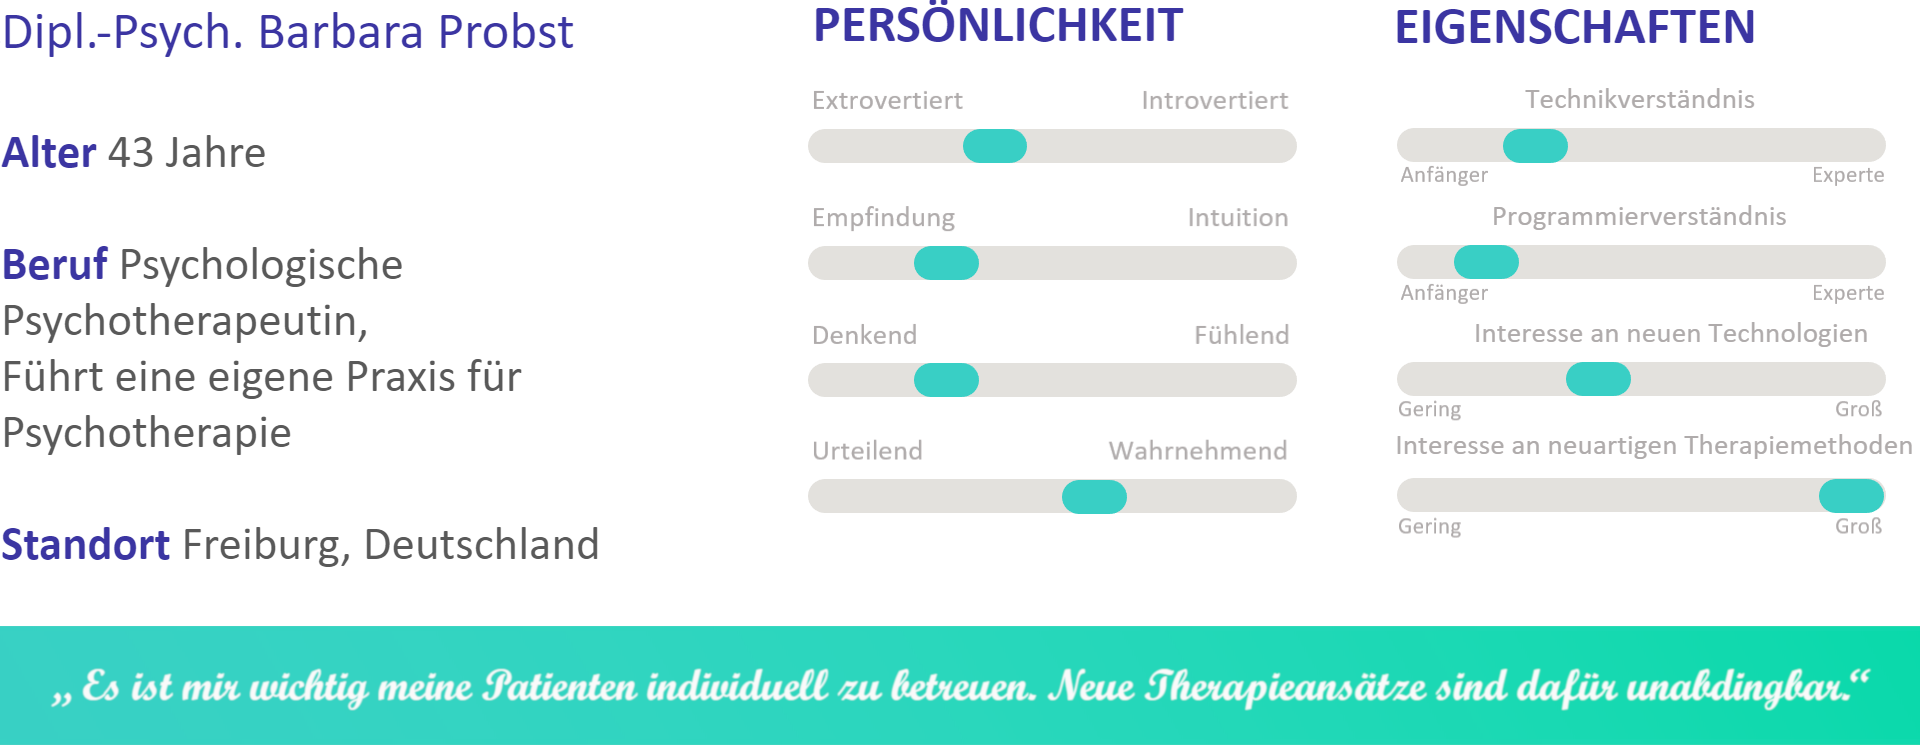
\includegraphics[width=1\textwidth]{pictures/therapeut}
\caption{Eckdaten der fiktiven Therapeutin \emph{Dipl.-Psych. Barbara Probst}}
\label{therapyBuilder}
\end{figure}

\paragraph{Profil}
Dipl.-Psych. Barbara Probst ist staatlich geprüfte psychologische Psychotherapeutin. Sie führt eine eigene Praxis. In dieser behandelt sie Patienten mit verschiedenen Störungen mit Krankheitswert. Ihr Spezialgebiet ist die Angststörung.

Sie wendet verschiedene Therapieansätze an. Diese werden individuell auf Persönlichkeit, Krankheitsverlauf und Symptomen des Patienten ausgewählt und zugeschnitten. Dabei nutzt sie altbewährte, wie auch neue Therapieansätze. Ihr Interesse gilt insbesondere neuartigen Therapiemethoden im Bereich der Angststörung. In ihrer Freizeit beschäftigt sie sich deshalb mit Fachjournalen. Sobald sie eine neue vielversprechende und geprüfte Therapiemethode entdeckt, notiert sie sich verschiedene Ansätze um diese auf geeignete Patienten zu übertragen. Dabei sind besonders Ansätze interessant, die neuartige Technologien verwenden.

Da ihr Stundenplan voll belegt ist muss die Übertragung neuer Therapiemethoden leicht und schnell gehen. Falls neue Technologien notwendig sind, sollen diese so leicht zu bedienen sein, dass kein Mehraufwand in Dokumentation und Planung entsteht. Außerdem ist es wichtig, dass eingesetzte Technologien wenig Aufwand und Expertenwissen benötigen um diese entsprechend einzurichten und zu bedienen.

\paragraph{Ziele}
\begin{itemize}
\item Austesten neuer Therapiemethoden
\item Einsatz neuer Technologien in Verbindung mit Psychotherapie
\item Neue Technologien sollten keinen Mehraufwand an Dokumentation darstellen
\item Neue Technologien und Therapien sollten keinen Mehraufwand an Planung darstellen
\item Einsatz neuer Therapiemethoden trotz wenig Zeit
\item Leicht integrierbar in den Alltag und das System eines Psychotherapeuten
\item Geringe Kosten in der Anwendung
\end{itemize}

\subsubsection{Patient}
Der Patient nutzt auf seinem Smartphone die \emph{TherapyBuilder}-App. Diese führt die Therapien aus, die dem Patienten vom Therapeut zugeordnet wurde. Betrachtet werden das Profil und die Ziele der fiktiven Patienten \emph{Jonas Vogt}.

\begin{figure}[h]
\centering
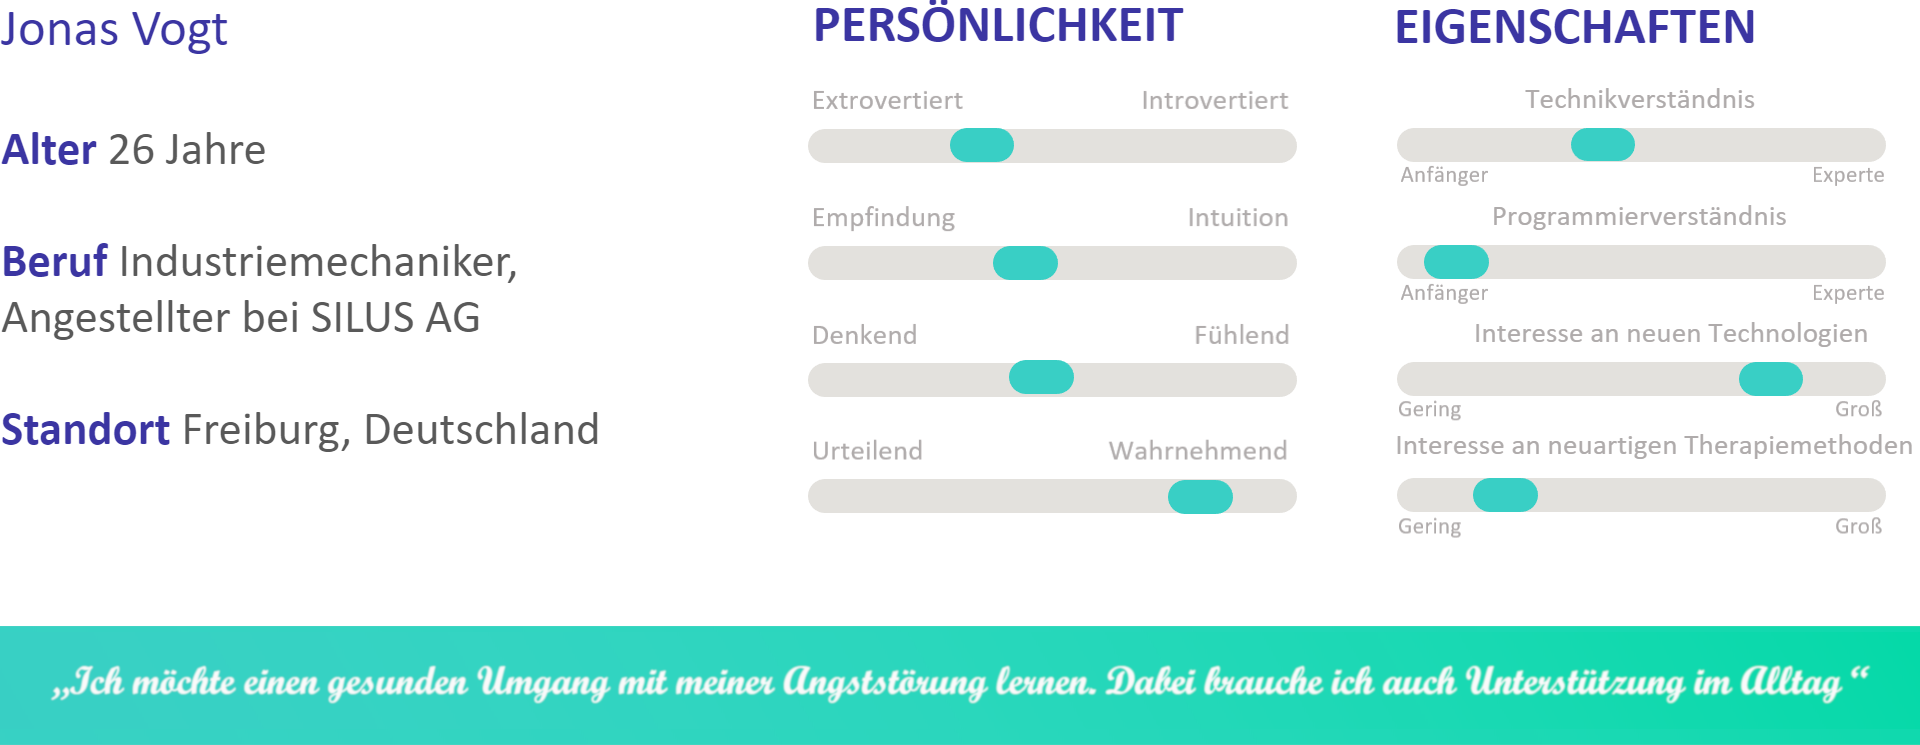
\includegraphics[width=1\textwidth]{pictures/patient}
\caption{Eckdaten des fiktiven Patienten \emph{Jonas Vogt}}
\label{therapyBuilder}
\end{figure}

\paragraph{Profil}
Jonas ist Industriemechaniker aus Freiburg. Er ist seit 3 Jahren Angestellter bei SILUS AG. Nach einem Jahr wurde er zum Schichtleiter befördert. Die Arbeit macht ihm sehr viel Freude. Er ist pflichtbewusst und nimmt seine Verantwortung als Schichtleitung ernst. Er beschäftigt sich in seiner Freizeit fast täglich mit neuen Strategien und Techniken für einen effizienten Schichtbetrieb. Aufgrund seines fachlichen Wissens und Engagements tauschen sich Arbeitskollegen wie Chefs gerne über neue Strategien mit ihm aus.

Neben seinem Beruf interessiert er sich für neue Technik-Gadgets, Spielekonsolen und Multimedia. In seiner Freizeit trifft er sich gerne mit Freunden zum Feiern, gemeinsamen Kochen aber auch zu gemütlichen Film und Spieleabenden. Er verabredet sich häufig über diverse Messenger und teilt über diese gerne Artikel über neue Technik-Gadgets.

Jonas hat eine Angststörung die als Begleiterscheinung eines Burn-outs während der Ausbildung auftrat.  Derzeit wartet er auf seine erste Therapiesitzung bei Dipl.-Psych. Barbara Probst. Während der Wartezeit nutzt er einen Chatbot. Diesen setzt er ein sobald er sich unwohl fühlt und die Angststörung auftritt. Seine Psychotherapeutin empfahl Jonas diesen Chatbot während der Wartezeit zu nutzen.

\paragraph{Ziele}
\begin{itemize}
\item Behandeln der Angststörung
\item Hilfe im Alltag wenn Angststörung auftritt
\item Einfache Anwendung der Hilfe
\item Hilfe jederzeit erreichbar
\item Hilfe leicht in Alltag integrierbar
\end{itemize}


\subsection{Studienbetrachtung}
Für die Anforderungsanalyse werden mehrere Studien betrachtet. Diese liegen der Firma \emph{movisens GmbH} in unterschiedlichen Formaten vor. Ablauf und Inhalte der jeweiligen Studie wurden in PowerPoint-Folien, Excel und Bildern, wie beispielsweise in Abbildung \ref{studie}, beschrieben. Jede Studie besitzt Inhalte, die in Form eines Chats umgesetzt werden könnten. Die Studien beinhalten Therapien, die in dieser evaluiert werden. Die Therapien setzen sich aus verschiedenen Stilmitteln zusammen. So finden sich Dialoge die aus Input und Output-Formaten bestehen. Die Input-Formate repräsentieren Formate, die dem Patienten angeboten werden um Daten einzugeben. Die Output-Formate beinhalten Formate, die dem Patienten angezeigt werden. Die Therapien bestehen aus Übungen, Interventionen und Selbstüberwachung.

\begin{figure}[h]
\centering
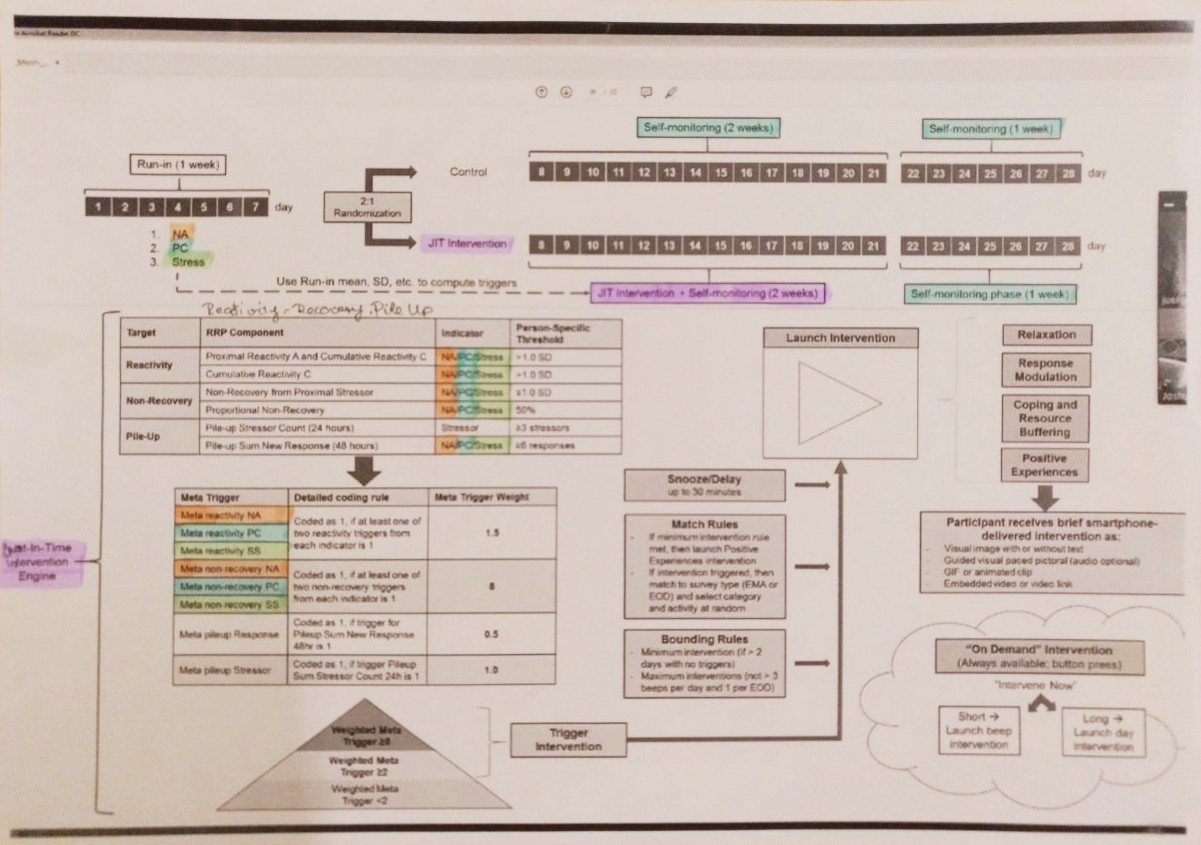
\includegraphics[width=1\textwidth]{pictures/studie}
\caption{Eckdaten des fiktiven Forschers \emph{Prof. Dr. Richard Weimer}}
\label{studie}
\end{figure}

Um eine Therapie umzusetzen, werden als Output-Formate Textausgaben, Video, Audio, und Bilder benötigt. Als Input-Formate für den Patienten werden Texteingabe, ganze Zahlen, rationale Zahlen, Likert-Skalen, visuelle Analogskalen, Einfach- wie Mehrfachauswahl, Zeiteingabe und eine Datumseingabe benötigt. 

Da auch Daten erhoben werden, benötigt es Variablen. In diesen werden Antworten und berechnete Werte gespeichert. Die Werte der Variablen können dem Patienten im Text präsentiert werden aber auch den Verlauf der Therapie beeinflussen. So können dem Patienten beispielsweise verschiedene Texte, Übungen oder Interventionen präsentiert werden. Die entsprechenden Inhalte werden zu unterschiedlichen Zeiten und Bedingungen ausgelöst. Auslöser können ein erreichtes Datum, vorgegebene Zeit, Therapeut, Patient oder verschiedene Bedingungen sein. Um diese Übersicht zu erhalten, wurde der zeitliche Ablauf der betrachteten Studien in einem Zeitstrahl abgebildet. Diese zeitliche Skizzierung wird in Abbildung \ref{studien} dargestellt.

\begin{figure}[h]
\centering
\includegraphics[width=1\textwidth]{pictures/studien}
\caption{Die zeitliche Abbildung verschiedener Studien in Form eines Zeitstrahls}
\label{studien}
\end{figure}


\subsection{Anforderungen}

\begin{figure}[h]
\centering
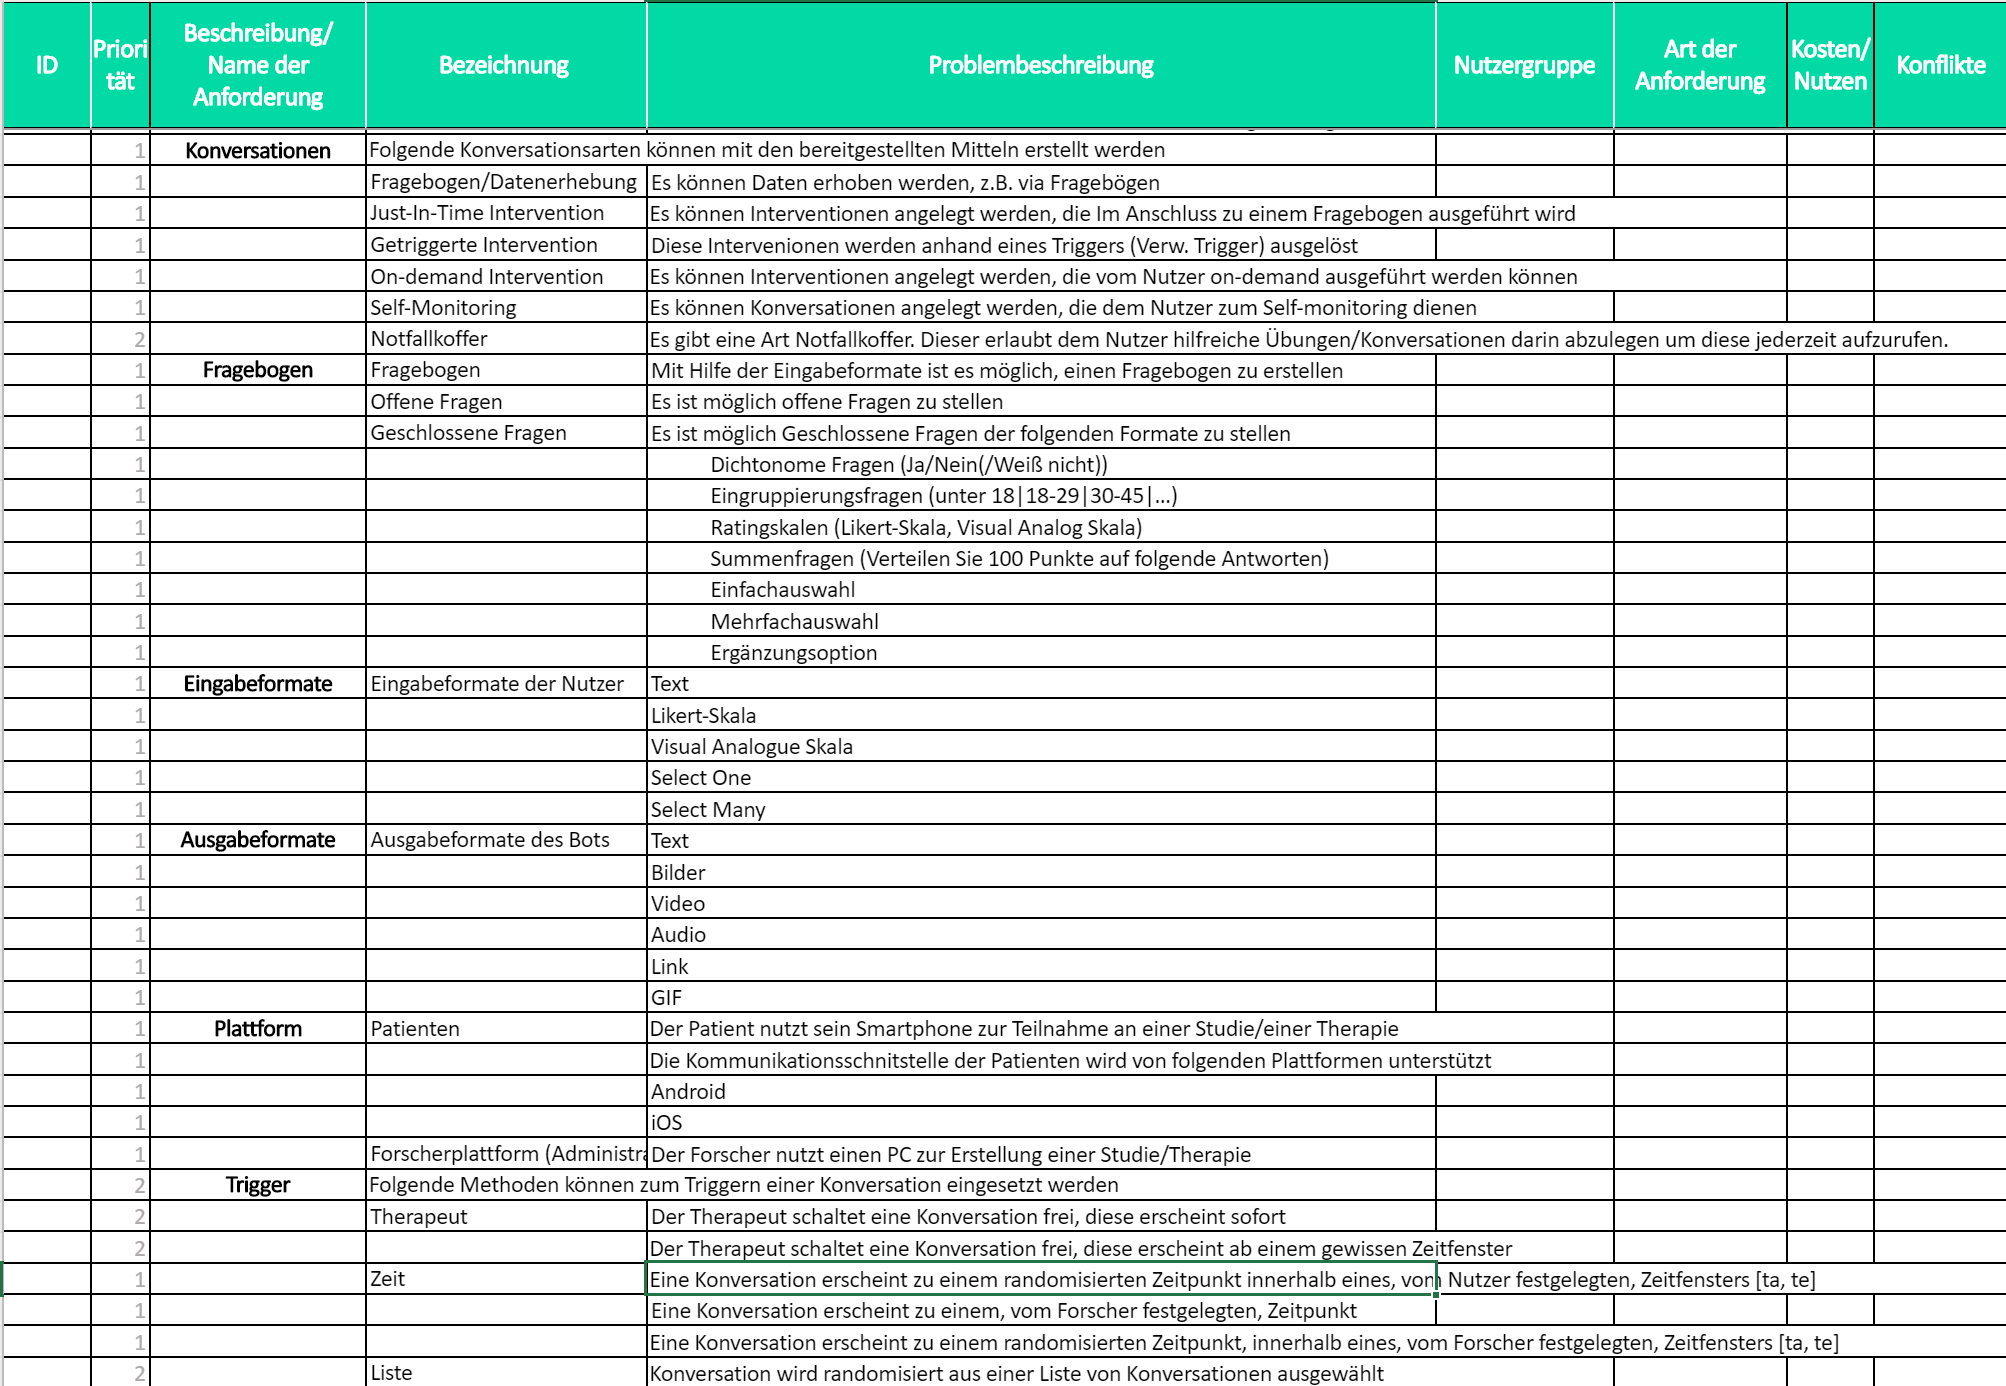
\includegraphics[width=1\textwidth]{pictures/anforderungen}
\caption{Die zeitliche Abbildung verschiedener Studien in Form eines Zeitstrahls}
\label{studien}
\end{figure}

\section{Ausarbeitung verschiedener Konzepte}

\subsection{Begriffsdefinitionen}

\subsection{Konzepte}
